% Created 2018-07-04 Wed 13:02
\documentclass[a4paper]{article}
\usepackage[utf8]{inputenc}
\usepackage[T1]{fontenc}
\usepackage{fixltx2e}
\usepackage{graphicx}
\usepackage{longtable}
\usepackage{float}
\usepackage{wrapfig}
\usepackage{rotating}
\usepackage[normalem]{ulem}
\usepackage{amsmath}
\usepackage{textcomp}
\usepackage{marvosym}
\usepackage{wasysym}
\usepackage{amssymb}
\usepackage{hyperref}
\tolerance=1000
\usepackage{minted}
\usepackage[margin=0.8in]{geometry}
\usepackage{amssymb,amsmath}
\usepackage{fancyhdr} %For headers and footers
\pagestyle{fancy} %For headers and footers
\usepackage{lastpage} %For getting page x of y
\usepackage{float} %Allows the figures to be positioned and formatted nicely
\restylefloat{figure} %and this command
\usepackage{hyperref}
\hypersetup{urlcolor=blue}
\usepackage{titlesec}
\setcounter{secnumdepth}{4}
\usepackage{minted}
\setminted{frame=single,framesep=10pt}
\chead{}
\rhead{\today}
\cfoot{}
\rfoot{\thepage\ of \pageref{LastPage}}
\usepackage[parfill]{parskip}
\usepackage{subfig}
\usepackage{pdfpages}
\hypersetup{colorlinks=true,linkcolor=black, citecolor=black}
\usepackage{framed}
\author{Nathan Hughes}
\date{\today}
\title{Comparing Domestication}
\hypersetup{
  pdfkeywords={},
  pdfsubject={},
  pdfcreator={Emacs 25.2.2 (Org mode 8.2.10)}}
\begin{document}

\maketitle

\section*{Information}
\label{sec-1}
\begin{itemize}
\item Significance testing for these values were done with one-way-ANOVA
\begin{itemize}
\item Bayesian estimations where used to fit the data to a normal distribution
\begin{itemize}
\item From 40,000 estimated data points, sampling was done on every 1000th point
\item These points were used for the ANOVA parameters.
\end{itemize}
\end{itemize}
\item Quantifying the differences where done with the Bayesian T-Test on estimated data.
\end{itemize}

\section*{Initial Thoughts}
\label{sec-2}


\begin{itemize}
\item Einkorn seems most interesting with significant changes across the board, with the exception of length(this has been previously reported?), length is also not significantly different in Emmer either.

\item Einkorn and Emmer both see significant changes in the length,depth,width ratio showing that this is a consistently significant change/indicator.

\item Einkorn and Emmer depth is significant too - I think John/Candida mentioned this being interesting as previous studies haven't been able to examine this trait fully?

\item Oddly, the surface area in Emmer isn't highly significant (<0.05,>0.01), yet the ratio trait (length,width,depth) is. Indicating it's perhaps a better measurement to consider when looking at 3D traits.

\begin{itemize}
\item Perhaps, like in previous studies, an interaction trait of lengthXwidth could be used for the marvin data, this might make a good proxy for comparing?
\end{itemize}

\item Numbers for the Emmer, spike-wise, are too low. With 3 data points for the wild, it's not sufficient to grasp anything meaningful
\begin{itemize}
\item The grain averages, I think are still useful enough
\end{itemize}

\item I don't know how best to interpret / relate the barley and it's meaning with wheat?
\end{itemize}

\clearpage
\section*{Summary Tables}
\label{sec-3}

\subsection*{\emph{T. boeticum} Vs. \emph{T. monococcum} (Einkorn)}
\label{sec-3-1}

\subsubsection*{Grains}
\label{sec-3-1-1}
\begin{longtable}{p{5cm}|r}
 & T. monococcum+T. beoticum\\
\hline
\endhead
\hline\multicolumn{2}{r}{Continued on next page} \\
\endfoot
\endlastfoot
length & 0.7045\\
width & < 0.001\\
depth & < 0.001\\
volume & < 0.001\\
surface\_area & < 0.001\\
length\_depth\_width & < 0.001\\
\end{longtable}



\subsubsection*{Spike Averages}
\label{sec-3-1-2}
\begin{longtable}{p{5cm}|r}
 & T. monococcum+T. beoticum\\
\hline
\endhead
\hline\multicolumn{2}{r}{Continued on next page} \\
\endfoot
\endlastfoot
mean\_length & 0.1848\\
mean\_width & < 0.001\\
mean\_depth & < 0.001\\
mean\_volume & < 0.001\\
mean\_surface\_area & < 0.001\\
mean\_length\_depth\_width & < 0.001\\
\end{longtable}


\clearpage
\subsection*{\emph{T. dicoccum} Vs. \emph{T. dicoccoides} (Emmer)}
\label{sec-3-2}

\subsubsection*{Grains}
\label{sec-3-2-1}
\begin{longtable}{p{5cm}|r}
 & T. dicoccum+T. dicoccoides\\
\hline
\endhead
\hline\multicolumn{2}{r}{Continued on next page} \\
\endfoot
\endlastfoot
length & 0.1106\\
width & 0.0141\\
depth & 0.0035\\
volume & < 0.001\\
surface\_area & 0.0401\\
length\_depth\_width & < 0.001\\
\end{longtable}


\subsubsection*{Spike Averages}
\label{sec-3-2-2}
\begin{longtable}{p{5cm}|r}
 & T. dicoccum+T. dicoccoides\\
\hline
\endhead
\hline\multicolumn{2}{r}{Continued on next page} \\
\endfoot
\endlastfoot
mean\_length & 0.4605\\
mean\_width & 0.3065\\
mean\_depth & < 0.001\\
mean\_volume & < 0.001\\
mean\_surface\_area & 0.192\\
mean\_length\_depth\_width & < 0.001\\
\end{longtable}



\clearpage
\subsection*{\emph{H. spontaneum} Vs. \emph{H. vulgare} (Barley)}
\label{sec-3-3}

\subsubsection*{Grains}
\label{sec-3-3-1}

\begin{longtable}{p{5cm}|r}
 & H. spontaneum+H. vulgare\\
\hline
\endhead
\hline\multicolumn{2}{r}{Continued on next page} \\
\endfoot
\endlastfoot
length & < 0.001\\
width & 0.2417\\
depth & 0.0001\\
volume & 0.6158\\
surface\_area & 0.0629\\
length\_depth\_width & 0.3784\\
\end{longtable}



\subsubsection*{Spike Averages}
\label{sec-3-3-2}
\begin{longtable}{p{5cm}|r}
 & H. spontaneum+H. vulgare\\
\hline
\endhead
\hline\multicolumn{2}{r}{Continued on next page} \\
\endfoot
\endlastfoot
mean\_length & 0.0067\\
mean\_width & 0.4459\\
mean\_depth & 0.0149\\
mean\_volume & 0.2436\\
mean\_surface\_area & 0.0575\\
mean\_length\_depth\_width & 0.2752\\
\end{longtable}





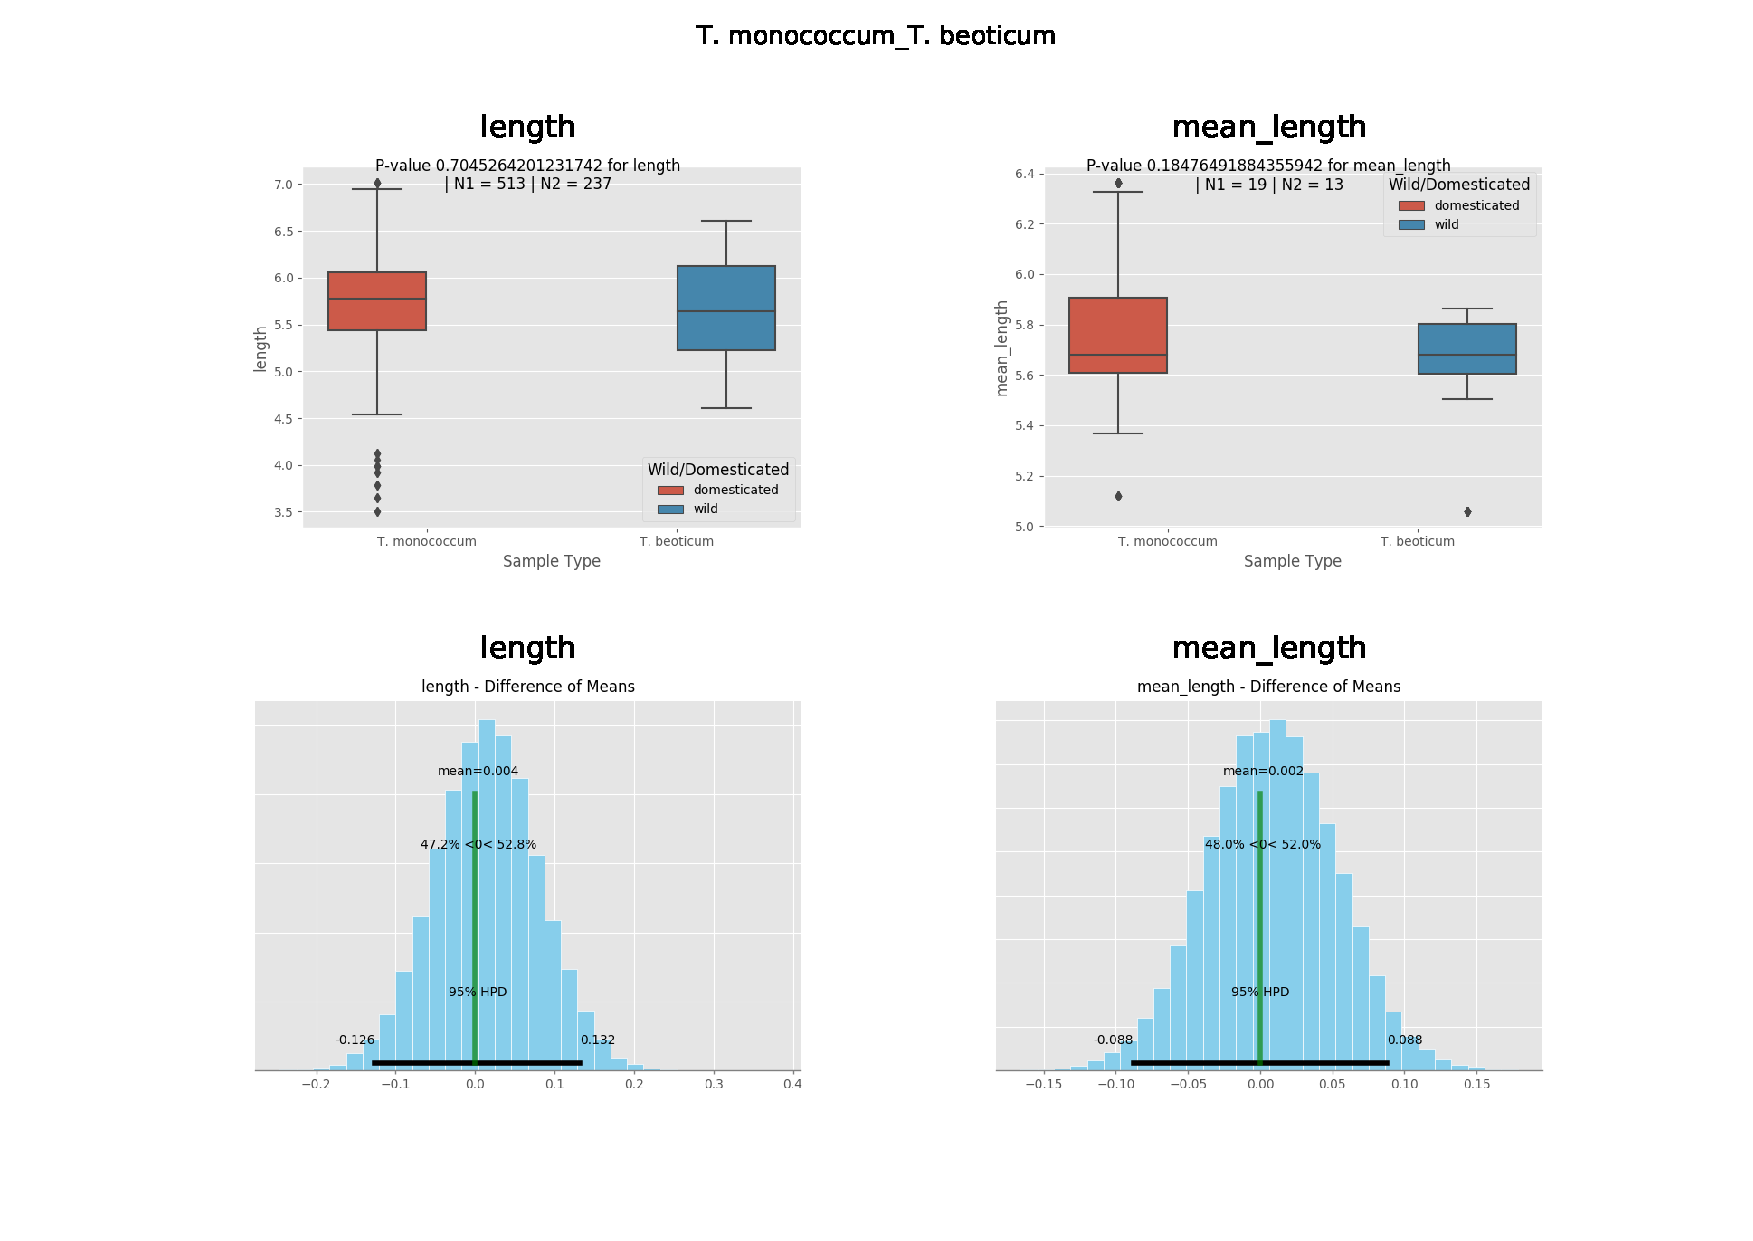
\includepdf[pages=-,angle=90,  pagecommand=\section{Einkorn}]{../Summaries/einkorn.pdf}


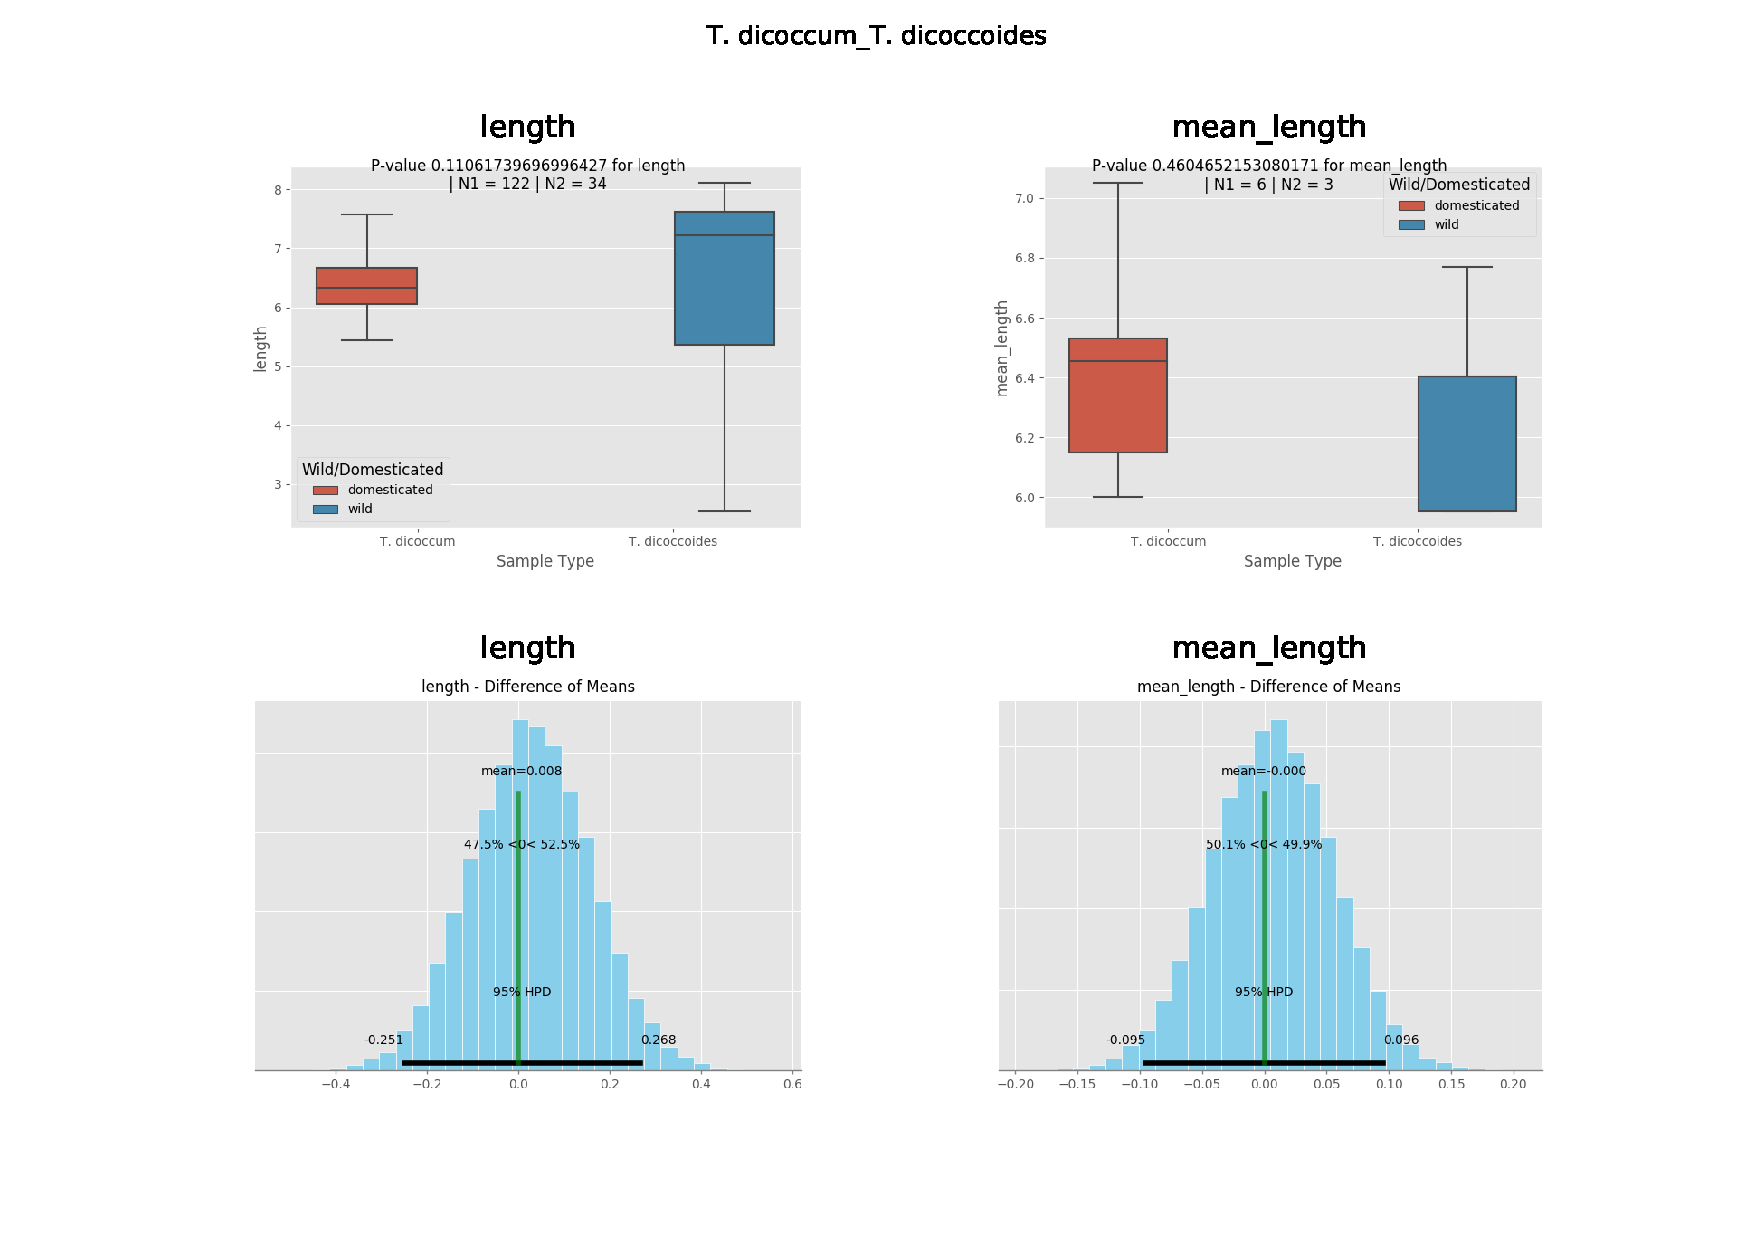
\includepdf[pages=-,angle=90,  pagecommand=\section{Emmer}]{../Summaries/emmer.pdf}


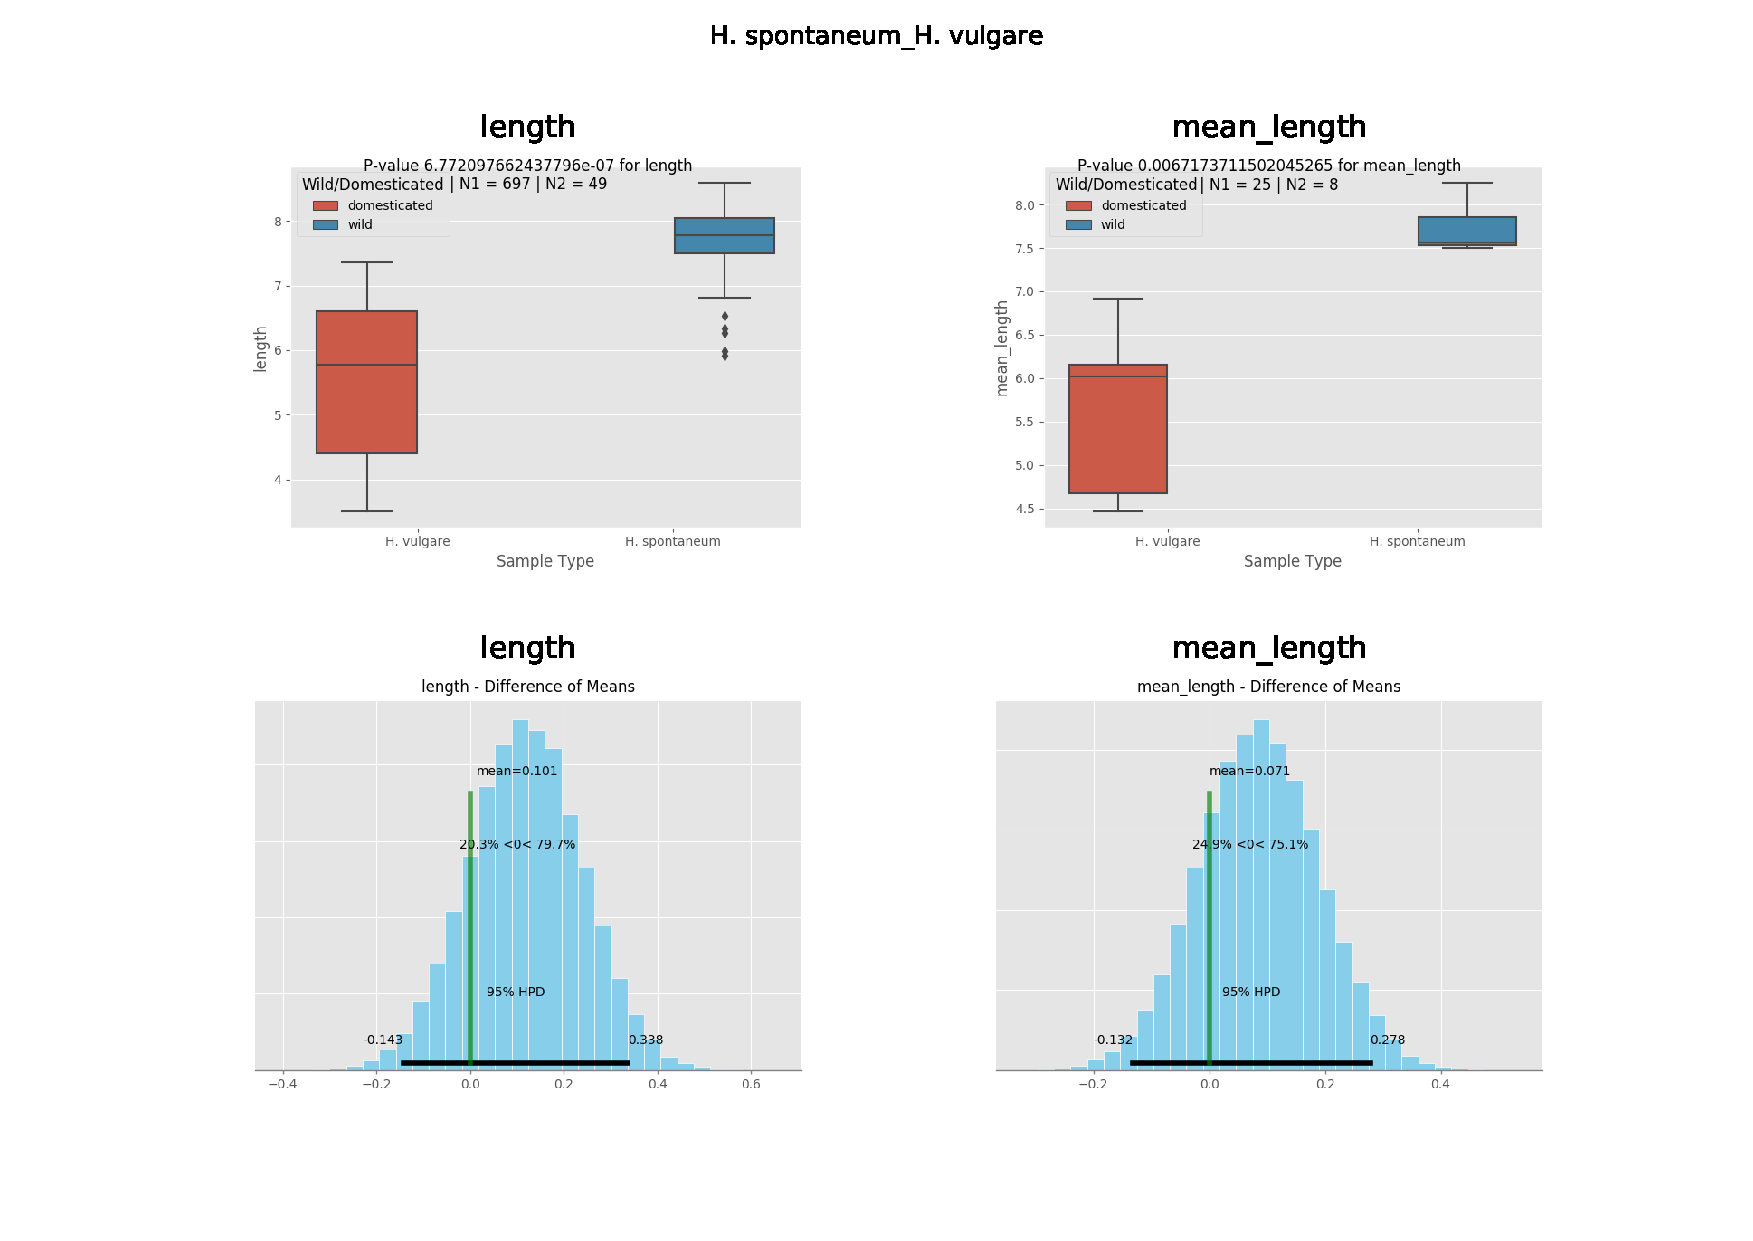
\includepdf[pages=-,angle=90,  pagecommand=\section{Barley}]{../Summaries/barley.pdf}
% Emacs 25.2.2 (Org mode 8.2.10)
\end{document}